
% This LaTeX was auto-generated from an M-file by MATLAB.
% To make changes, update the M-file and republish this document.

\documentclass{article}
\usepackage{graphicx}
\usepackage{color}
\usepackage{listings}
\usepackage[framed]{mcode}
\usepackage{fullpage}
\usepackage{amsmath}
\usepackage[utf8x]{inputenc}
\usepackage{import}
\usepackage{setspace}
\usepackage{hyperref}
\definecolor{lightgray}{gray}{0.5}
\setlength{\parindent}{0pt}

\begin{document}

    
    
%\section*{}


\title{BE 521: Homework 5 \\{\normalsize Vision} \\{\normalsize Spring 2021}}
\author{42 points}
\date{Due: Tuesday, 03/02/2021 10 pm}
\maketitle \textbf{Objective:} Visual responses and likelihood


\begin{center} \author{Jal Mahendra Panchal \\
  \normalsize Collaborators: Sam Gaardsmoe \\}
\end{center}


\subsection*{V1 Dataset}
In this homework, you will work with data from 18 cells recorded from mouse primary visual cortex (also known as V1). Cells in this area are responsive to specific angles. Hence, a common stimulation paradigm is to show the subject a sinusoidal grating drifting at a specific angle (see Figure 1).
\begin{figure}[h!]
 \centering
 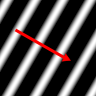
\includegraphics[width=48px]{figs/grad30.png}
 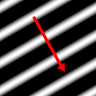
\includegraphics[width=48px]{figs/grad60.png}
 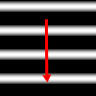
\includegraphics[width=48px]{figs/grad90.png}
 \caption{Example sinusoidal drifting grating at (in order left to right) 30, 60, and 90 degrees, where the red arrows shows the direction of the drift.}
\end{figure}
This data was collected and graciously provided by Daniel Denman in the Contreras Lab, University of Pennsylvania. The file \verb|mouseV1.mat| contains two variables: \verb|neurons|, a cell array representing all the times that each of the 18 cells fired a spike during the approximately 7 minute long experiment, and \verb|stimuli|, which provides the time (first column, in milliseconds) that a given angle (second column) was presented in this experiment.  Note that each stimulus in \verb|stimuli| is presented for exactly 2 seconds, after which a gray screen is presented for approximately 1.5 seconds (therefore each trial is approximately 3.5 seconds in duration.)
\section{Stimulus Response (11 pts)}
In this section, you will explore the response of the cells to different stimulus angles.
\begin{enumerate}
 \item How many unique grating angles, \textit{m}, are there in \verb|stimuli|? (1 pt)

$\textbf{Answer 1.1} \\$
\begin{lstlisting}
mv1 = load('mouseV1.mat');
\end{lstlisting}
\begin{lstlisting}
unique_angles = unique(mv1.stimuli(:,2));
size(unique_angles,1)
\end{lstlisting}

\color{lightgray} \begin{lstlisting}
ans =

    12

\end{lstlisting} \color{black}
There are 12 unique grating angles in the stimuli, 0, 30, 60, 90, 120, 150, 180, 210, 240, 270, 300, 330. Though 6 of the angles \ensuremath{>}= 180 will essentially have the same grating pattern as the 6 below 180 deg.

 \item A \emph{tuning curve} is frequently used to study the response of a neuron to a given range of input stimuli. To create tuning curves for this data, calculate the average number of spikes each cell fires in response to each grating angle. Store the result in an $18\times m$ dimensional matrix, where each element represents the response of a single neuron to a particular input stimulus angle, with each neuron assigned a row and each angle assigned a column. In a $2\times 2$ Matlab subplot, plot the tuning curve for the first four cells.  Place the stimulus angle on the x-axis and the number of spikes on the y-axis.  (6 pts)

$\textbf{Answer 1.2} \\$
\begin{lstlisting}
tuning_curve_data = zeros(18, 12);
num_stim_angle = zeros(12,1);
%loop through all trials of each of the 12 angles
for i = 1 : size(unique_angles,1)

    ang = unique_angles(i);
    %find the trials for each angle
    stim_index = find(mv1.stimuli(:,2)==ang);

    num_stim_angle(i) = size(stim_index,1);

    %loop through all trials and check how many triggers for each cell is
    % within the duration of a trial
    for j= 1: size(stim_index,1)

        idx = stim_index(j);
        %find the start and stop time of each trial
        % here we are approximating to secs as the question says approx 1.5
        % wait after a 2 sec show of image11
        start_time_ms = mv1.stimuli(idx,1)/1000;
        start_time_s = round(start_time_ms,1);
        end_time_s = start_time_s + 3.5; % 3.5 sec window

        %cheecking if the trigger for any neuron lies within time range of
        %a given trial
        for k = 1:18
            trig_time_s = round([mv1.neurons{k}]./1000,1);
            num_trig = size(find(trig_time_s>= start_time_s & trig_time_s <=end_time_s),1);

            tuning_curve_data(k,i) = tuning_curve_data(k,i) + num_trig;
        end

    end
end
\end{lstlisting}
\begin{lstlisting}
%Calculating average for each grating angle
tuning_curve_avg = tuning_curve_data ./num_stim_angle';
\end{lstlisting}
\begin{lstlisting}
%plot
figure();
subplot(2,2,1)
plot(unique_angles, tuning_curve_avg(1,:), 'Linewidth', 2);
title('Neuron 1')
xlabel('Grating angle')
ylabel('Average number of spikes')
xlim([0,360])

subplot(2,2,2)
plot(unique_angles, tuning_curve_avg(2,:), 'Linewidth', 2);
title('Neuron 2')
xlabel('Grating angle')
ylabel('Average number of spikes')
xlim([0,360])

subplot(2,2,3)
plot(unique_angles, tuning_curve_avg(3,:), 'Linewidth', 2);
title('Neuron 3')
xlabel('Grating angle')
ylabel('Average number of spikes')
xlim([0,360])

subplot(2,2,4)
plot(unique_angles, tuning_curve_avg(4,:), 'Linewidth', 2);
title('Neuron 4')
xlabel('Grating angle')
ylabel('Average number of spikes')
xlim([0,360])

suptitle('Average spikes vs grating angle for different neurons')
\end{lstlisting}


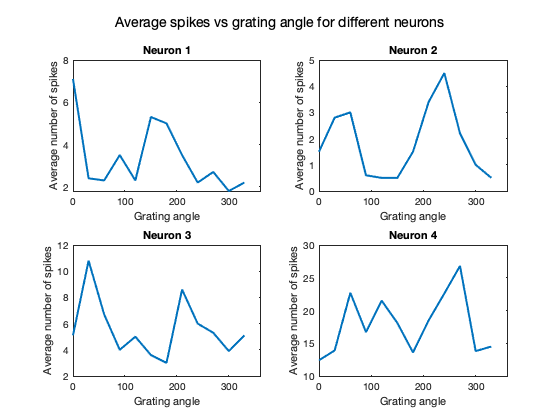
\includegraphics [width=5in]{jalp_hw5_01.png}

  \begin{enumerate}
   \item Look through the tuning response curves of each of the 18 cells.  How reasonable is it to assume that the response of a given cell to angle $\theta$ is the same as its response to angle $\theta+180$? Include at least a few tuning curves to back up your answer. (2 pts)

$\textbf{Answer 1.2a} \\$
Based on how the grating patterns look, the pattern for $\theta$ and $\theta+180$ do look similar in most cases , the patterns are jagged due to low number of samples. The response for stimuli images for $\theta$ and $\theta+180$ is similar as the stimuli are the same when flipped by 180 so the neuron would respond identically to both the angles. $\\$ Here are a few examples of neurons that show this phenomenon.
\begin{lstlisting}
%plot
figure();
subplot(2,2,1)
plot(unique_angles, tuning_curve_avg(2,:),'Linewidth', 2);
xline(180)
title('Neuron 2')
xlabel('Grating angle')
ylabel('Average number of spikes')
xlim([0, 360])


subplot(2,2,2)
plot(unique_angles, tuning_curve_avg(6,:), 'Linewidth', 2);
xline(180)
title('Neuron 6')
xlabel('Grating angle')
ylabel('Average number of spikes')
xlim([0, 360])

subplot(2,2,3)
plot(unique_angles, tuning_curve_avg(7,:), 'Linewidth', 2);
xline(180)
title('Neuron 7')
xlabel('Grating angle')
ylabel('Average number of spikes')
xlim([0, 360])

subplot(2,2,4)
plot(unique_angles, tuning_curve_avg(14,:), 'Linewidth', 2);
xline(180)
title('Neuron 14')
xlabel('Grating angle')
ylabel('Average number of spikes')
xlim([0, 360])

suptitle('Showing symmetry in response for $\theta$ and $\theta+180$')
\end{lstlisting}


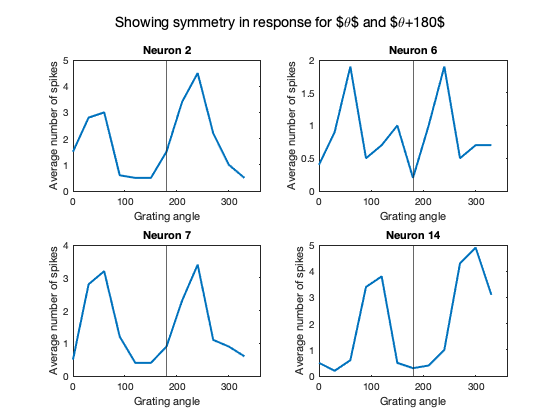
\includegraphics [width=5in]{jalp_hw5_02.png}

   \item Does this assumption have any physiological justification (given what you know about the types of cells in V1)? (2 pts)

$\textbf{Answer 1.2b} \\$
Yes, the neurons in V1 would have high sensitivity for orientation of the grating images(stimuli). As the orientation of the images for $\theta$ and $\theta + 180$ would look the same, the neurons will not be able to differentiate between the two images and fire similarly for both. Thus we see this behavior of response of a neuron being similar for $\theta$ and $\theta + 180$.

  \end{enumerate}
\end{enumerate}
\section{Neural Decoding (31 pts)}
Suppose we would like to work backwards - that is, for a given neural response, can we predict what the grating angle was? This process is called ``neural decoding,'' and is especially of interest to the BCI motor control community (as we'll see in a later homework).
In this section, we will try out an approach which is detailed in Jazayeri \& Movshon 2006 \footnote{A copy of this paper is included if you are curious, but we walk you through the method in this homework.}.
The method we will use involves finding the maximum likelihood of
the data. \\ \\
Here, the data is the number of spikes $s_i$ that cell $i$ fires when the subject sees a stimulus with grating angle $\theta$. One way to think about our likelihood function is to ask the question ``given a stimulus angle $\theta$, how many spikes would I expect this cell to fire?'' We can represent this number of spikes $s_i$ using a Poisson process with parameter $f_i(\theta)$ for a stimulus $\theta$, where $f_i$ represents neuron $i$'s tuning function.
A Poisson distribution is often used to model count data that occurs at a constant rate, and in this case the rate is given by $f_i(\theta)$. In other words, our likelihood function $L_i(\theta)$ for each neuron $i$ is the probability $p(s_i|\theta)$ of neuron $i$ firing $s_i$ spikes for a given value of $\theta$.
The idea in this method is to calculate the log likelihood\footnote{log = natural log unless other    wise specified} function of each neuron and then add them all together to get the log likelihood function of the entire population of ($n$) neurons. We often work with the $\emph{log}$ likelihood because it allows adding of probabilities instead of multiplying, which can lead to numerical problems.
\begin{align*}
p(s_i|\theta) \sim &\; Pois(f_i(\theta)) = \frac{f_i(\theta)^{s_i}}{s_i!} e^{-{f_i(\theta)}} \tag{Poisson probability density}\\
\L_i(\theta) =&\; p(s_i|\theta) \tag{Likelihood of a given neuron firing at $s_i$}\\
\L(\theta) = &\; \prod_{i=1}^n p(s_i|\theta) \tag{Joint likelihood of all n neurons}\\
\log \L(\theta) = &\;\sum_{i=1}^n \log L_i(\theta) = \sum_{i=1}^n \log p(s_i|\theta)  \tag{Take log}\\
\propto &\;  \sum_{i=1}^n s_i \log f_i(\theta) \tag{evaluation of PDF and simplifying}
\end{align*}
Thus, we can define the log likelihood for each neuron $i$ as the log of its tuning curve $f_i(\theta)$ times the number of spikes $s_i$ it fires for a particular stimulus $\theta$, and the population log likelihood is simply the summation across all cells. This tells us that, given a set of tuning curves $f_i(\theta)$, we can compute the likelihood of observing our data $s$.
But we already have those tuning curves for each cell from question 1.2, so all we need to know for a new (hidden) stimulus is how many spikes each neuron fires. Let $\mathbf{s}$ be the $n$-dimensional column vector of the number of spikes each cell fires after the subject is presented with a new stimulus $\theta'$ and let $\mathbf{F}$ be the $n\times m$ matrix representing the tuning curves of each neuron at each of the $m$ stimuli (for us, $m$ is the number of stimuli between 0 and 150 degrees because we assume that all neurons respond equally to $\theta$ and $\theta+180$ degrees.)  We can then compute the log likelihood of the new stimulus $\theta'$ easily using the inner product of $\mathbf{s}$ and $\mathbf{F}$: \verb|L = s'*log(F)|.
\begin{enumerate}
 \item Compute the matrix \verb|F| by recalculating the tuning curves you calculated in question 1.2 using only the \textbf{first 70} trials (this is akin to our ``training'' data). You will use the remaining 50 trials (as ``testing'' data) to make predictions. Make a histogram of the number of stimulation angles for the first 70 trials to ensure that each angle (0 to 150) is presented at least a few times. (4 pts)

$\textbf{Answer 2.1} \\$
\begin{lstlisting}
%seprating training data
mv1_train = mv1;
mv1_train.stimuli = mv1_train.stimuli(1:70,:);
\end{lstlisting}
\begin{lstlisting}
tuning_curve_train = zeros(18, 12);
num_stim_angle_train = zeros(12,1);
%loop through all training trials of each of the 12 angles
for i = 1 : size(unique_angles,1)

    ang = unique_angles(i);
    %find the trials for each angle
    stim_index = find(mv1_train.stimuli(:,2)==ang);

    num_stim_angle_train(i) = size(stim_index,1);

    %loop through all trials and check how many triggers for each cell is
    % within the duration of a trial
    for j= 1: size(stim_index,1)

        idx = stim_index(j);
        %find the start and stop time of each trial
        % here we are approximating to secs as the question says approx 1.5
        % wait after a 2 sec show of image11
        start_time_ms = mv1.stimuli(idx,1)/1000;
        start_time_s = round(start_time_ms,1);
        end_time_s = start_time_s + 3.5; % 3.5 sec window

        %cheecking if the trigger for any neuron lies within time range of
        %a given trial
        for k = 1:18
            trig_time_s = round([mv1_train.neurons{k}]./1000,1);
%             temp_ = [temp_, find(trig_time_s>= start_time_s & trig_time_s <=end_time_s)];
            num_trig = size(find(trig_time_s>= start_time_s & trig_time_s <=end_time_s),1);

            tuning_curve_train(k,i) = tuning_curve_train(k,i) + num_trig;
        end

    end
end
\end{lstlisting}
\begin{lstlisting}
%folding the matrix to combine angles above 180
tuning_curve_train = tuning_curve_train(:, 1:6) + tuning_curve_train(:,7:12);
num_stim_angle_train = (num_stim_angle_train(1:6) + num_stim_angle_train(7:12))';
tuning_curve_train_avg = tuning_curve_train ./ num_stim_angle_train;
\end{lstlisting}
\begin{lstlisting}
%plotting histogram
% After combining the trials above and below 150 deg, we get the following
% histogram for number of trials for each angle. \\
figure();
angles_trian_folded = [mv1.stimuli((mv1_train.stimuli(:,2)<180),2)',...
    (mv1.stimuli((mv1_train.stimuli(:,2)>=180),2)-180)'];
ax = histogram(angles_trian_folded, 30).Parent;
set(ax, 'XTick', 0:30:150);
title('Number of trials for each grating angle, training set, n=70')
xlabel('Grating angle')
ylabel('Number of trials')
\end{lstlisting}


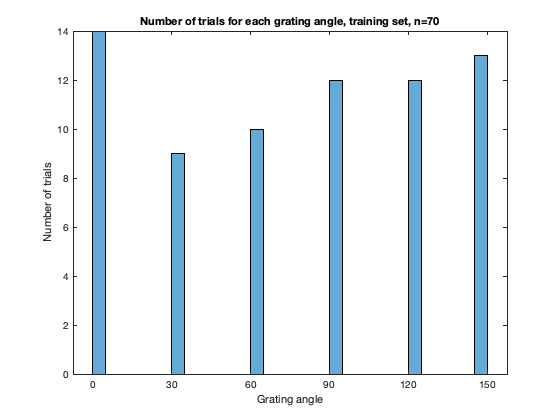
\includegraphics [width=5in]{jalp_hw5_03.png}

 \item For the 50 ``testing'' trials, compute a $n \times 50$ matrix \verb|S| where each row
represents the number of spikes one neuron fired in response to a each of the 50 trials. With this, you can easily compute the log likelihood functions for all the trials at
once with the command: \verb|L_test = S'*log(F)|. (Hint: add a small number to \verb|F| to avoid taking the log of 0)
  \begin{enumerate}
	\item Plot the likelihood functions for the first four testing trials in a $2\times 2$ subplot. In the title of each plot, give the trial number (1, 2, 3, or 4) and the true stimulation angle. Make sure to label your axes correctly. (5 pts)

$\textbf{Answer 2.2a} \\$
\begin{lstlisting}
%seprating testing data
%testing set starts from 71st trial
mv1_test = mv1;
mv1_test.stimuli = mv1_test.stimuli(71:120,:);
\end{lstlisting}
\begin{lstlisting}
%computing testing set
spike_count_test = zeros(18, 50);
%loop through all 50 testing trials
for j= 1:50

    idx = j;

    %find the start and stop time of each trial
    % here we are approximating to secs as the question says approx 1.5
    % wait after a 2 sec show of image11
    start_time_ms = mv1_test.stimuli(idx,1)/1000;
    start_time_s = round(start_time_ms,1);
    end_time_s = start_time_s + 3.5; % 3.5 sec window

    %cheecking if the trigger for any neuron lies within time range of
    %a given trial
    for k = 1:18
        trig_time_s = round([mv1_test.neurons{k}]./1000,1);
        num_trig = size(find(trig_time_s>= start_time_s & trig_time_s <=end_time_s),1);

        spike_count_test(k,j) = spike_count_test(k,i) + num_trig;
    end

end
\end{lstlisting}
\begin{lstlisting}
%calculating l_test using tuning curve of average spikes per grating angle
%from training data
l_test = spike_count_test'*log(tuning_curve_train_avg);
\end{lstlisting}
\begin{lstlisting}
%ploting l_test
figure();
subplot(2,2,1)
n = 1;
ang = mv1_test.stimuli(n,2);
plot(unique_angles(1:6), l_test(n,:), 'Linewidth', 2);
title(['Test Trial :', num2str(n), '  True angle :',num2str(ang)])
xlabel('Grating angle')
ylabel('Log likelihood function')
xlim([0, 150])


subplot(2,2,2)
n = 2;
ang = mv1_test.stimuli(n,2);
plot(unique_angles(1:6), l_test(n,:), 'Linewidth', 2);
title(['Test Trial :', num2str(n), '  True angle :',num2str(ang),'(=0)'])
xlabel('Grating angle')
ylabel('Log likelihood function')
xlim([0, 150])

subplot(2,2,3)
n = 3;
ang = mv1_test.stimuli(n,2);
plot(unique_angles(1:6), l_test(n,:), 'Linewidth', 2);
title(['Test Trial :', num2str(n), '  True angle :',num2str(ang)])
xlabel('Grating angle')
ylabel('Log likelihood function')
xlim([0, 150])

subplot(2,2,4)
n = 4;
ang = mv1_test.stimuli(n,2);
plot(unique_angles(1:6), l_test(n,:), 'Linewidth', 2);
title(['Test Trial :', num2str(n), '  True angle :',num2str(ang)])
xlabel('Grating angle')
ylabel('Log likelihood function')
xlim([0, 150])

suptitle('Log Likelihood Function for test stimuli')
\end{lstlisting}


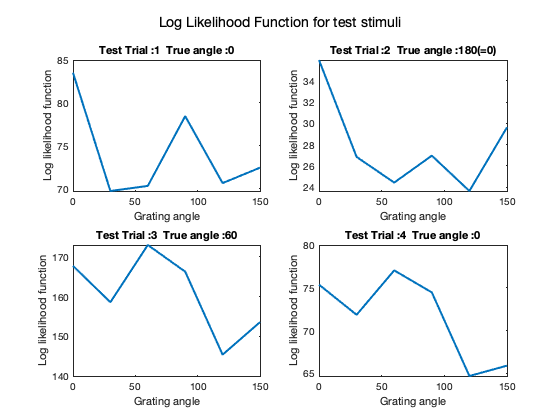
\includegraphics [width=5in]{jalp_hw5_04.png}

	\item How well do these four likelihood functions seem to match the true stimulation angle? Explain in a few sentences. (3 pts)

$\textbf{Answer 2.2b} \\$
For the trials 1, 2 and 3 the prediction is quite accurate, the true grating angle is correctly predicted by the angle with the highest probability from the likelihood function which is 0 for trial 1, 0(or 180) for trial 2 and 60 for trial 3. $\\$ For trial 4, the max value from the likelihood funtion is obtained for 60 deg but the grating angle is 0 deg. This is probably due to the higher sensitivity of the 4th neuron to 60 deg as compared to 0 deg. Also, the 4th neuron has the most number of spikes for a stimulus so it dominates the prediction of the likelihood function.

	\item Compute the maximum likelihood estimate (MLE) for each of
	the 50 trials. This is another way of asking which angle $\theta$ has the highest probability.
	\[ \hat{\theta}_{MLE} = \arg\max_\theta\; L(\theta) = \arg\max_\theta\; \log L(\theta) \]
	In what percentage of the 50 trials did your MLE correctly predict the stimulation angle [0-150]? (5 pts)

$\textbf{Answer 2.2c} \\$
\begin{lstlisting}
%calculating max probability
[max_l, max_l_indx] = max(l_test, [],2);
pred_ang = unique_angles(max_l_indx,1);

%finding the accuracy of MLE
angles_test_folded = zeros(50,1);
for i = 1:50
    if mv1_test.stimuli(i,2) < 180
        angles_test_folded(i) = mv1_test.stimuli(i,2);
    else
        angles_test_folded(i) = mv1_test.stimuli(i,2)-180;
    end
end


pred_accuracy = (size(find(pred_ang == angles_test_folded),1)/50)*100
\end{lstlisting}

\color{lightgray} \begin{lstlisting}
pred_accuracy =

    44

\end{lstlisting} \color{black}
The MLE predicted 44\% of the trials or 22 of the 50 test trials correctly.

	\item
	In a few sentences, discuss how well this method worked for predicting the input angle from the response of the 18 neurons.  What might you change in the experimental protocol to try and get a better prediction? (3 pts)
	\end{enumerate}

$\textbf{Answer 2.2d} \\$
At 44\% percent, the MLE algorith did a good job for prediction if we compare it to the binomial distribution of expected accuracy of 16.7 \% .\$\ensuremath{\backslash}\ensuremath{\backslash}\$ But from a pratical application, the accuracy is below 50\% so it gets the angle wrong most of the time which seems like not a good result. This can be improved by training from a much larger training sample as compared to 70 trials in this case. Also, some neurons fire/spike much more than other neurons, they dominate and bias the prediction of the algorithm. Depending on if we prefer this or if want to weigh the spikes for each neuron equally, we can normalize the number if spikes for each nueron depending on the average spike of that neuron for all angles.

  \item It is important to show that your findings are not a result of chance. One way to demonstrate this is using a ``permutation test.'' Here, we will perform a permutation test by randomly reassigning new grating angles to the 50 test responses and then calculating how often the new grating angles match the true stimulation angles.
	\begin{enumerate}
	 \item Simulate the chance prediction (the ``null'' distribution) by randomly reassigning the stimulation angles 1000 times.  For each permutation, calculate the percent accuracy of each label. Create a histogram of the 1000 accuracy measurements for the null distribution. Add a red vertical line with the accuracy calculated from using the Jazayeri method above. (4 pts)

$\textbf{Answer 2.3a} \\$
\begin{lstlisting}
%calculating probability of random chance
null_dist_acc = zeros(1000,1);
for i = 1:1000

   random_test_trial = zeros(50,1);
   %finding a random set of angles for 50 trials
   for j = 1:50

       %fixing seed for randomization
       seed = (i-1)*50+j;
       rng(seed);

       r_idx = randperm(6,1);
       r_ang = unique_angles(r_idx);
       random_test_trial(j) = r_ang;
   end

   acc_n = (size(find(random_test_trial == angles_test_folded),1)/50)*100;
   null_dist_acc(i) = acc_n;
end
\end{lstlisting}


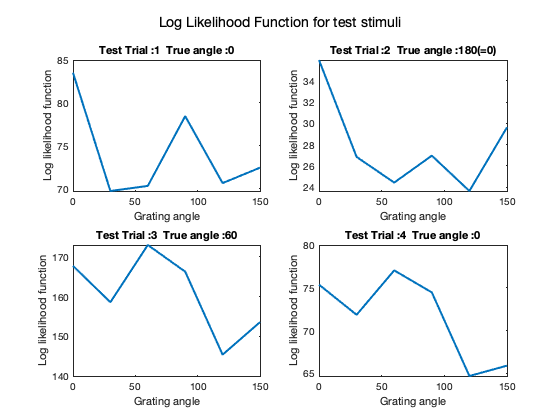
\includegraphics [width=5in]{jalp_hw5_05.png}
\begin{lstlisting}
%Plotting null distribution
figure();
histogram(null_dist_acc);
xline(pred_accuracy, 'color', 'red', 'Linewidth', 2);
title('Null distribution for 50 trials for 6 grating angles, n = 1000');
legend('Null' , 'MLE')
xlabel('Accuracy %')
ylabel('Number of experiments')
\end{lstlisting}


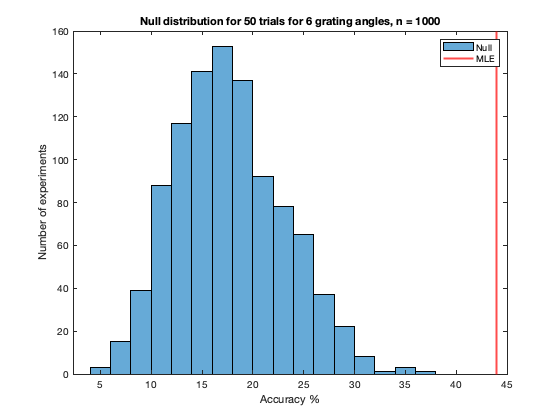
\includegraphics [width=5in]{jalp_hw5_06.png}

	 \item Is the null distribution what you expected? Explain. (1 pt)

$\textbf{Answer 2.3b} \\$
Yes, for a large sample size like 1000 we would expect the null hypothesis to have a bell shaped distribution of binomial distibution or an approximately normal distribution for given parameters. $\\$ Comparing the results to a binomial distribution of 50 trials with a probability of 1/6 for each trial we get similarly shaped curve with a mean close to 1/6 or 16.66\%
\begin{lstlisting}
%Example Binomial distribution
%50 trials with a p of 1/6 for each
y  = binopdf(0:50, 50, 1/6);
figure();
plot(0:2:100, y,  'Linewidth', 2);
xlim([0,50])
title('Binomial distribution n=50, p=1/6')
xlabel('Accuracy %')
ylabel('Probabilty density')
\end{lstlisting}


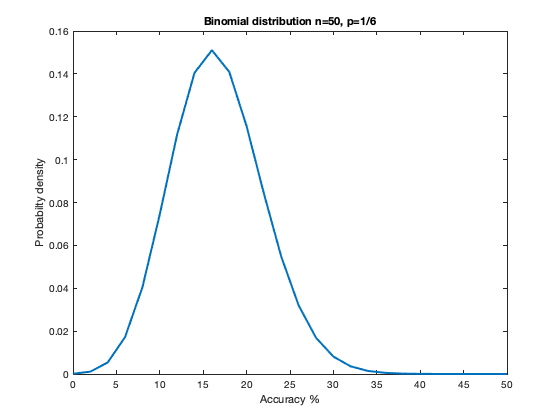
\includegraphics [width=5in]{jalp_hw5_07.png}

	\item What is the probability that your actual accuracy measurement comes from the null-distribution?  That is, calculate the fraction of permutation samples with accuracy \emph{more extreme} relative to the mean of the null distribution (less than your measurement if your value is less than the mean, or more than your measurement if your value is more than the mean). (2 pts)

$\textbf{Answer 2.3c} \\$
\begin{lstlisting}
samples_great_meas = null_dist_acc(null_dist_acc>pred_accuracy);
p_val_meas = (size(samples_great_meas, 1)/1000)*100
\end{lstlisting}

\color{lightgray} \begin{lstlisting}
p_val_meas =

     0

\end{lstlisting} \color{black}
From our null hypothesis distribution, 0\% of the values are above the predicted probability of 44\% from MLE. This is expected as the MLE has a much higher accuracy than the null distribution and it would never predict it.

	\item What would the probability be if your accuracy had been 25\%? (1 pt)

$\textbf{Answer 2.3d} \\$
\begin{lstlisting}
%calculating probabilty that 25% is predicted from null hypothesis
test_val = 25;
samples_great_test = null_dist_acc(null_dist_acc>test_val);
p_val_test = (size(samples_great_test, 1)/1000)*100
\end{lstlisting}

\color{lightgray} \begin{lstlisting}
p_val_test =

    7.2000

\end{lstlisting} \color{black}
In this iteration of radomization for null distribution, we get a p-value of 7.2\% for a 25\% accurary in the null hypothesis.

	\item What is this value typically called? (1 pt)

$\textbf{Answer 2.3e} \\$
This value of probability of finding the observed accuracy or more extreme given null hypothesis is true is called the p-value

	\end{enumerate}
  \item The tuning curves and neuron responses to a new trial were calculated using the number of spikes each neuron fired after the stimulation. But what if a particular neuron just happens to fire a lot and fires even more when it gets a stimulus to which it's tuned? Those neurons could ``swamp'' the log likelihood estimate given in Equation 1 by virtue of just having a larger average $s_i$ and $f_i(\theta)$.
  How might we correct for this type of behavior?  Suggest a possible method. (2 pts)

$\textbf{Answer 2.4} \\$
Here we are considering that all the neurons should have the same weightage in number of spikes/fires per stimuli for the calculation. To do this we can normalize the number of spikes for each neuron by the average spike of that neuron for for the whole range of angles, this way the multi spike of some neurons dont bias the log weights as compared to neuron that are orientation sensitive but have fewer spikes for a stumulus. $\\$ We could also explore different weights like a cosinosoidal weights instead of a log weight for the tuning function as touched upton in Jazayeri \& Movshon 2006 for calculating likelihood of direction of motion and explore different ways to weight the spikes and normalize for each neuron.

\end{enumerate}
\end{document}




\end{document}
    
